\chapter{Introduction}

\vspace{-1cm}

\paragraph{} This chapter has seven parts: (1) Background of the Study, (2) Statements of the Problem, (3) Theoratical Framework, 
            (4) Conceptual Framework, (5) Scope and Limitations, (6) Significance of the Study, and (7) Definition of Terms.

\paragraph{} Part one, Background of the Study, gives an overview as to which the research problem was anchored.

\paragraph{} Part two, Statement of the Problem, identifies the main problem and enumerates the specific problems which the study hoped to answer.

\paragraph{} Part three, Theoretical Framework, discussed the relevance of the variables in the identified theory, concept or principle to 
            the research problem.

\paragraph{} Part four, Conceptual Framework, presents the paradigm of the study.

\paragraph{} Part five, Scope and Limitations, specifies the scope and coverage of the study in terms of purpose, research design, 
            research instruments and statistical tools employed in the study.

\paragraph{} Part six, Significance of the Study, presents the possible contributions and the specific application of knowledge that 
            might be gained from the result of the study.

\paragraph{} Part seven, Definition of Terms, contains the conceptual and operational definitions of key terms used in the study.

\section{Background of the Study}
\paragraph{} As the ocean covers over 70\% of the Earth's surface, presenting a vast and complex environment ripe for exploration and study. 
            Sea surface drones offer a valuable tool for navigating water bodies, collecting data, and conducting research across various disciplines. 
            Unmanned surface vehicles (USVs) equipped with autonomous navigation capabilities have become pivotal in various applications, particularly 
            in water environments.

\paragraph{} Early USVs were also called ASC; Autonomous Surface Craft (ASCs)which were first developed at the MIT Sea Grant College Program in 1993 and 
            were designed for various missions. Aptly named ARTEMIS,the vessel was a scale replica of a fishing trawler used as a platform capable of 
            testing the navigation and control systems required by an ASC. Later on a new ASC ACES(Autonomous Coastal Exploration System) was developed 
            during 1996 and 1997(Justin E. Manley 2008)

\paragraph{} Further adaptation of USV in the early 20th century saw the development of remotely controlled USVs used for mine detection and target 
            practice. World War II further spurred advancements, with nations utilizing USVs for reconnaissance and explosive delivery. Post-war, 
            oceanographic research embraced USVs for data collection and underwater exploration. Notably, the bathyscaphe Trieste, equipped with a 
            rudimentary autopilot, famously reached the deepest point in the Earth's oceans in 1960( National Museum of the U.S. Navy)
          
\paragraph{} The 1990s witnessed a surge in commercial applications, with USVs employed for offshore oil and gas exploration, pipeline inspections, and 
            aquaculture monitoring. The 21st century has seen a continued proliferation of USVs, with advancements in sensor technology, autonomous 
            navigation systems, and communication capabilities propelling their capabilities further.

\paragraph{} However, while traditional methods for marine data collection involve time-consuming, expensive, and potentially risky manual operations,
            unmanned surface vehicles (USVs) offer a compelling alternative. These vehicles promise efficient, cost-effective, and safe data collection 
            across vast areas. However, current USV technology faces three key hurdles: high cost due to complex hardware and software, limited 
            accessibility due to user interfaces and maintenance requirements, and navigation challenges in dynamic aquatic environments. This study aims 
            to address these limitations by developing a modular unmanned surface drone with a focus on simplified maintenance, affordability, and 
            interchangeable components that can be easily switched.

\paragraph{} Empirical testing conducted as part of this research, quantifying the water surface drone's ability to reach predefined target positions, 
            serves as a critical quantitative assessment of the system's accuracy. The results obtained will offer data ensuring the navigational 
            reliability of the drone.

\paragraph{} The drones modular design enables adaptation on sea applications based on specific needs, seamlessly integrating communication modules, 
            lifesaving equipment, or various sensors as required. This adaptability ensures tailored responses to emergency situations and varied data 
            collection demands. 


\section{Statement of the Problem}
\paragraph{} How accurate is the Modular Self-Navigating unmanned surface drone when moving from point of origin to the user inputted coordinates?

\section{Hypothesis}
\paragraph{} Drone accuracy will be high and can effectively navigate to the user supplied coordinates.

\section{Theoratical Framework}
\paragraph{} From a control systems perspective, the Drone leverages feedback mechanisms and advanced algorithms to achieve autonomous navigation and 
            mission execution. This dictates the drone's ability to gather environmental data, make real-time decisions, and dynamically adjust its 
            actions based on sensor readings and mission parameters. Furthermore, the modular design aligns with the principles of modular robotics, 
            emphasizing the benefits of independent, interchangeable components. This enables tailored configurations for diverse tasks, offering 
            adaptability to various environments and operational needs. Additionally, the drone can be understood through the distributed systems theory, 
            which emphasizes the coordination of multiple agents towards a common goal. In this context, the modular components act as individual agents 
            collaborating to make the sea surface drone function. This theory guides the design of communication protocols and inter-module coordination 
            algorithms, essential for seamless collaboration and collective task execution. By integrating these theories, drone development can benefit 
            from established principles in control, modularity, and distributed systems, leading to a robust, adaptable, and efficient platform for maritime 
            operations.

\section{Conceptual Framework}
\begin{figure}[ht]
\begin{center}
\begin{tikzpicture}[NODE/.style={rectangle, draw=black!60, fill=white!0, very thick, minimum size = 20mm}]

\node[NODE]   (input)   {User-supplied Coordinates};
\node[NODE]   (throughput) [right = of input] {\parbox{120px}{\centering Data processing algorithm \\ \vspace{10pt} Sensor Data (GPS and Magnetometer)}};
\node[NODE]   (output) [right = of throughput] {\parbox{120px}{\centering Adjusted navigation data \\ \vspace{10pt} Motor control signals}};

\node [above = of input] {Input};
\node [above = of throughput] {Throughput};
\node [above = of output] {Output};

\draw[->, very thick] (input.east) to node[right] {} (throughput.west);
\draw[->, very thick] (throughput.east) to node[right] {} (output.west);

\end{tikzpicture}
\end{center}

\caption{Conceptual Framework}
\label{fig:ConceptualFramework}
\end{figure}

\paragraph{} Figure \ref{fig:ConceptualFramework} shows the conceptual framework on how the drone functions. To discuss briefly; user provides geographical
           coordinates or destination data to the ESP-32 onboard the sea surface drone. Magnetometer and GPS sensors collect real-time data regarding the 
           drone's current position, orientation, and the magnetic field. The ESP-32 employs a navigation algorithm that processes user input and sensor 
           data from gps and magnetometer.

\paragraph{} Continuous feedback loop adjusts the drone's path in real-time based on the latest sensor data, ensuring adaptability to various sea disturbances.


\vspace{2cm}

\begin{center}
\bf Objectives:
\end{center}

{\bf General Objectives:}
\paragraph{} -- To design an ESP-32 based water surface drone with autonomous navigation capabilities using GPS and Magnetometer

{\bf Specific Objectives:}
\paragraph{} -- To construct an easy to use and maintainable water surface drone system
\paragraph{} -- To test the accuracy of the sea surface drone to reach the target 

\section{Significance of the Study}
\paragraph{} Developing a modular water surface drone equipped with autonomous navigation capabilities holds significant value. The widespread adoption of
            such drones requires accessible construction and upkeep, making them viable tools for various users. Evaluating the drone's accuracy in reaching
            target positions offers crucial empirical data, validating its reliability and paving the way for more practical applications. This project 
            contributes to the progress of sea surface drone technology, potentially impacting research initiatives in oceanography, environmental monitoring, 
            and more. Furthermore, being easy to reproduce fosters broader use, democratizing access to this technology.

\section{Scope and Limitations of the Study}
\paragraph{} The research concentrates on assessing the accuracy of the drone's navigation, particularly in reaching user-provided coordinates, with a focus
            on real-time adjustments and adaptability to various water disturbances.  The drone is limited to a navigation algorithm that checks and corrects
            for its navigational pathing on loop. Said algorithm is only designed for relatively small distances as it doesn't take into account the curvature 
            of the earth and the distance measured by the algorithm is assuming a straight line and not a part of the Great Circle.

\vspace{0.5cm}
\begin{figure}[ht]
\centering
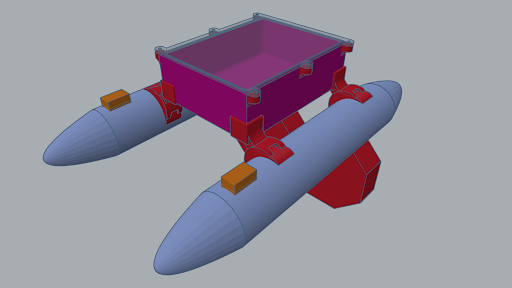
\includegraphics[scale = 0.60]{assets/3d_model_complete.png}
\caption{CAD Model}
\label{fig:3dModelComplete}
\end{figure}

\paragraph{} The study does not consider the potential challenges posed by capsizing due to strong tidal waves or encountering large obstructing objects
            in the ocean. Furthermore, the research does not extensively explore the intricate legal and regulatory frameworks governing unmanned surface 
            drones, instead prioritizing an in-depth examination of the technical aspects related to navigation.

\paragraph{} While the study’s primary focus is on navigation accuracy, the drone is inherently modular(Figure \ref{fig:3dModelComplete}). This modular 
            design enables the replacement of various components to meet the specific requirements of future users, enhancing its versatility and 
            adaptability in different scenarios.

\section{Definition of Terms}
{\begin{itemize}
  \item ESP32 -- low-cost, low-power system-on-chip (SoC) microcontrollers designed by Espressif Systems. Widely used in various applications such as 
        IoT (Internet of Things), home automation, wearables, and industrial automation due to its versatility, low cost, and built-in Wi-Fi and Bluetooth
        connectivity. It is commonly programmed using the Arduino IDE or the Espressif IDF (IoT Development Framework).
  \item Shroud -- refers to 3d printed components that covers and protects the propeller from marine debris. Secures brushless motor in place.
  \item Pontoon -- refers to 3d printed components; Provides the drone with enough buoyancy to keep afloat on water.
  \item Enclosure -- refers to 3d printed waterproof containers housing electronic components. 
  \item Bracket -- refers to 3d printed components; Design includes 6 pieces connecting the shroud to the pontoon and the pontoon to the enclosure.
\end{itemize}}